\documentclass[11pt]{article}

\usepackage[letterpaper,margin=0.68in,headheight=15pt,footskip=28pt]{geometry}
\usepackage[T1]{fontenc}
\usepackage{lmodern}
\usepackage{microtype}
\usepackage{amsmath,amssymb}
\usepackage{booktabs,tabularx,array,multirow}
\usepackage{enumitem}
\usepackage[table]{xcolor}
\usepackage{tikz}
\usetikzlibrary{positioning,arrows.meta}
\usepackage[most]{tcolorbox}
\usepackage{multicol}
\usepackage{titlesec}
\usepackage{fancyhdr}
\usepackage{lastpage}
\usepackage{needspace}
\usepackage[hidelinks]{hyperref}

\definecolor{Navy}{HTML}{15324A}
\definecolor{Teal}{HTML}{118A8A}
\definecolor{Sky}{HTML}{DFF3F4}
\definecolor{Gold}{HTML}{F2B134}
\definecolor{GoldLight}{HTML}{FFF4D6}
\definecolor{Coral}{HTML}{E76F51}
\definecolor{CoralLight}{HTML}{FCE8E2}
\definecolor{Ink}{HTML}{24323D}
\definecolor{SoftGray}{HTML}{F4F6F7}
\definecolor{MidGray}{HTML}{667782}
\definecolor{AnswerBlue}{HTML}{1E5AA8}
\definecolor{Green}{HTML}{3A8D5D}

\color{Ink}
\setlength{\parindent}{0pt}
\setlength{\parskip}{4pt}
\setlist[itemize]{leftmargin=1.35em,itemsep=2pt,topsep=3pt}
\setlist[enumerate]{leftmargin=1.65em,itemsep=5pt,topsep=4pt}
\renewcommand{\arraystretch}{1.22}

\titleformat{\section}{\Large\bfseries\color{Navy}}{}{0pt}{}[\vspace{-3pt}\color{Teal}\titlerule]
\titleformat{\subsection}{\large\bfseries\color{Teal}}{}{0pt}{}
\titleformat{\subsubsection}{\normalsize\bfseries\color{Navy}}{}{0pt}{}
\titlespacing*{\section}{0pt}{12pt}{7pt}
\titlespacing*{\subsection}{0pt}{9pt}{4pt}

\pagestyle{fancy}
\fancyhf{}
\lhead{\textcolor{MidGray}{AP Statistics: Lessons 1.1--1.3}}
\rhead{\textcolor{MidGray}{Quiz Study Guide}}
\cfoot{\textcolor{MidGray}{\thepage\ of \pageref{LastPage}}}
\renewcommand{\headrulewidth}{0.3pt}

\newtcolorbox{bigidea}[1]{
  enhanced,breakable,colback=Sky,colframe=Teal,boxrule=0.9pt,
  arc=2mm,left=3mm,right=3mm,top=2mm,bottom=2mm,
  title={#1},fonttitle=\bfseries\color{Navy},coltitle=Navy,
  attach boxed title to top left={xshift=2mm,yshift=-2mm},
  boxed title style={colback=Sky,colframe=Teal,boxrule=0pt}
}

\newtcolorbox{trapbox}[1][Common trap]{
  enhanced,breakable,colback=CoralLight,colframe=Coral,boxrule=0.9pt,
  arc=2mm,left=3mm,right=3mm,top=2mm,bottom=2mm,
  title={#1},fonttitle=\bfseries,coltitle=Coral,
  attach boxed title to top left={xshift=2mm,yshift=-2mm},
  boxed title style={colback=CoralLight,colframe=Coral,boxrule=0pt}
}

\newtcolorbox{formulabox}[1]{
  enhanced,breakable,colback=GoldLight,colframe=Gold,boxrule=0.9pt,
  arc=2mm,left=3mm,right=3mm,top=2mm,bottom=2mm,
  title={#1},fonttitle=\bfseries\color{Navy},coltitle=Navy,
  attach boxed title to top left={xshift=2mm,yshift=-2mm},
  boxed title style={colback=GoldLight,colframe=Gold,boxrule=0pt}
}

\newtcolorbox{answerbox}[1][Answer]{
  enhanced,breakable,colback=white,colframe=AnswerBlue,boxrule=0.7pt,
  arc=1.5mm,left=3mm,right=3mm,top=2mm,bottom=2mm,
  title={#1},fonttitle=\bfseries,coltitle=AnswerBlue,
  attach boxed title to top left={xshift=2mm,yshift=-2mm},
  boxed title style={colback=white,colframe=AnswerBlue,boxrule=0pt}
}

\newcommand{\term}[1]{\textbf{\textcolor{Teal}{#1}}}
\newcommand{\key}[1]{\textbf{\textcolor{Navy}{#1}}}
\newcommand{\ans}[1]{\textcolor{AnswerBlue}{#1}}
\newcommand{\workline}{\vspace{0.33in}\hrulefill}
\newcommand{\shortline}{\rule{1.35in}{0.4pt}}
\newcommand{\choicebox}{\raisebox{0.1ex}{\tikz\draw[Ink,line width=0.5pt] (0,0) rectangle (0.14,0.14);}}
\newcolumntype{Y}{>{\raggedright\arraybackslash}X}
\newcolumntype{C}{>{\centering\arraybackslash}X}

\begin{document}

\begin{tcolorbox}[enhanced,colback=Navy,colframe=Navy,arc=3mm,boxrule=0pt,left=6mm,right=6mm,top=5mm,bottom=5mm]
{\Huge\bfseries\color{white} AP Statistics Quiz Study Guide}\par
\vspace{2pt}
{\Large\color{Gold} Lessons 1.1--1.3: Categorical Data Foundations}\par
\vspace{5pt}
{\color{white}Statistical studies $\boldsymbol{\rightarrow}$ categorical tables $\boldsymbol{\rightarrow}$ graphs and association}
\end{tcolorbox}

\begin{center}
\begin{tabularx}{0.96\textwidth}{>{\bfseries\color{Navy}}l Y}
Built from: & Lesson 1.1, 1.2, and 1.3 notes, homework, and answer keys\\
Best use tonight: & Read the concept pages, cover the answers, complete the practice set, then grade yourself from the key.\\
Quiz goal: & Name the correct denominator, compare conditional percentages, and explain conclusions in context.\\
\end{tabularx}
\end{center}

\begin{bigidea}{The complete quiz checklist}
By the end, you should be able to do each task without notes.
\begin{multicols}{2}
\begin{itemize}[label=\textcolor{Teal}{\checkmark}]
  \item Identify individuals and variables.
  \item Classify variables as categorical or quantitative.
  \item Distinguish population, sample, and census.
  \item Distinguish prospective and retrospective studies.
  \item State a realistic limitation; avoid causal claims.
  \item Find frequency and relative frequency.
  \item Read marginal, joint, and conditional values.
  \item Choose explanatory and response variables.
  \item Decide whether two categorical variables are associated.
  \item Read side-by-side and segmented bar graphs.
  \item Explain the height, width, and area in a mosaic plot.
  \item Turn percentages back into counts, and counts back into a total.
  \item Say which comparisons a graph does and does not support.
  \item Identify misleading scales and misleading pictures.
\end{itemize}
\end{multicols}
\end{bigidea}

\subsection*{A focused 60-minute plan}
\begin{tabularx}{\textwidth}{>{\bfseries\color{Teal}}p{0.75in} Y}
0--15 min & Memorize the vocabulary and denominator rules in the concept section.\\
15--30 min & Redo the two class-data worked examples without looking at the blue solutions.\\
30--50 min & Complete the mixed practice sets without using the answer key.\\
50--60 min & Grade with the answer key. Redo only the questions you missed.\\
\end{tabularx}

\newpage
\section{Lesson 1.1: Statistical Studies}

\begin{bigidea}{What a statistical study does}
A statistical study collects data from a \term{sample} to answer an \term{investigative question} about a \term{population}. A conclusion is strongest when the sample represents the population well.
\end{bigidea}

\begin{tabularx}{\textwidth}{>{\bfseries\color{Navy}}p{1.28in} Y p{2.05in}}
\toprule
Term & Meaning & Question to ask\\
\midrule
Individual & One object or person described by the data & ``Who or what is each row about?''\\
Variable & A characteristic recorded for each individual & ``What changes from individual to individual?''\\
Population, $N$ & The entire group the conclusion is about & ``Who do researchers want to understand?''\\
Sample, $n$ & The subset from which data were actually collected & ``Who was actually measured?''\\
Census & Data collected from every individual in the population & ``Was everyone in that population included?''\\
\bottomrule
\end{tabularx}

\begin{trapbox}[Wording a variable correctly]
A variable must describe the recorded value for \emph{each individual}. Write ``whether or not an adult owns a pet,'' not merely ``owning a pet.'' Write ``reaction time in milliseconds,'' not merely ``reaction.''
\end{trapbox}

\subsection{Categorical vs. quantitative variables}
\begin{tabularx}{\textwidth}{>{\bfseries\color{Navy}}p{1.35in} Y Y}
\toprule
Type & Definition & Examples from the lessons\\
\midrule
Categorical & Values are category names or group labels. Arithmetic on the labels is not meaningful. & Drinks coffee daily (yes/no); long or short walk; developed disease (yes/no); preferred class\\
Quantitative & Values are numerical measurements or counts. Arithmetic is meaningful. & Reaction time; stress score; number of steps; exam score; hours worked\\
\bottomrule
\end{tabularx}

\begin{trapbox}[Numbers can still be categorical]
A jersey number, ZIP code, or student ID is a label, so it is categorical. Ask whether averaging the values would make sense.
\end{trapbox}

\subsection{Prospective vs. retrospective}
\begin{center}
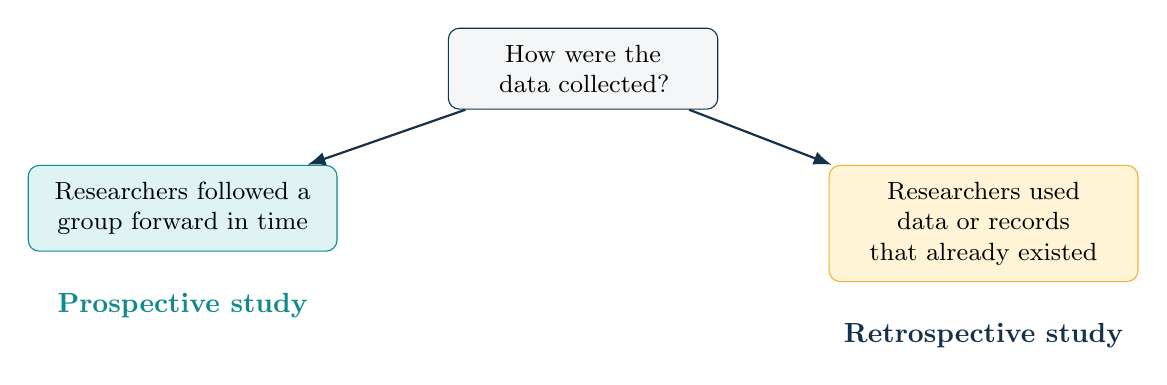
\begin{tikzpicture}[node distance=7mm and 14mm,every node/.style={font=\small}]
  \node[draw=Navy,rounded corners,fill=SoftGray,inner sep=6pt,text width=3.0cm,align=center] (q) {How were the data collected?};
  \node[draw=Teal,rounded corners,fill=Sky,inner sep=6pt,text width=3.5cm,align=center,below left=of q] (p) {Researchers followed a group forward in time};
  \node[draw=Gold,rounded corners,fill=GoldLight,inner sep=6pt,text width=3.5cm,align=center,below right=of q] (r) {Researchers used data or records that already existed};
  \node[below=4mm of p,font=\bfseries\color{Teal}] {Prospective study};
  \node[below=4mm of r,font=\bfseries\color{Navy}] {Retrospective study};
  \draw[-{Latex},thick,Navy] (q) -- (p);
  \draw[-{Latex},thick,Navy] (q) -- (r);
\end{tikzpicture}
\end{center}

\key{Evidence words matter:} ``monitored for 8 years'' supports prospective; ``examined existing survey data'' supports retrospective.

\subsection{Limitations and conclusions}
Common valid limitations in the provided materials include:
\begin{itemize}
  \item a short measurement period may not represent usual behavior;
  \item self-reported responses may be inaccurate;
  \item the sample may not represent the target population;
  \item another variable may explain the association (confounding);
  \item an observational study shows association, not cause and effect.
\end{itemize}

\begin{trapbox}[Safe conclusion language]
Say ``was associated with,'' ``tended to,'' or ``was more likely.'' Do not say one variable \emph{caused} the other unless a well-designed experiment supports that claim.
\end{trapbox}

\newpage
\section{Lesson 1.2: Analyzing Categorical Data}

\subsection{One categorical variable}
\begin{tabularx}{\textwidth}{>{\bfseries\color{Navy}}p{1.35in} Y Y}
\toprule
Display & What it shows & Key rule\\
\midrule
Bar graph & Frequency or relative frequency for categories & Bars are separated; a frequency axis must start at 0.\\
Pie chart & Each category's share of the whole & All slices total 100\%.\\
\bottomrule
\end{tabularx}

\begin{formulabox}{Frequency language --- and how to run it backwards}
\[
\text{relative frequency of a category}
=\frac{\text{frequency in that category}}{\text{total number of individuals}}
\qquad
\text{percent}=100\%(\text{relative frequency})
\]
Solve for whichever piece is missing:
\[
\text{count}=(\text{relative frequency})(\text{total}),
\qquad
\text{total}=\frac{\text{count}}{\text{relative frequency}}.
\]
\key{From the notes:} 9 students chose Music and Music was 30\% of the sample, so the total sampled is $\ans{9/0.30=30\text{ students}}$; a missing category count is then $30-(6+9+4+4)=\ans{7}$.
\end{formulabox}

\begin{trapbox}[Name the individuals first]
``The 30 major league baseball teams'' are the individuals; league (categorical), stadium capacity (quantitative), wins last season (quantitative), and whether or not the team made the playoffs (categorical) are the variables. Individuals are not always people.
\end{trapbox}

\subsection{Two-way tables: choose the denominator first}
Suppose the rows are categories of variable $A$ and the columns are categories of variable $B$.

\begin{center}
\begin{tabular}{l|cc|c}
 & $B_1$ & $B_2$ & Total\\ \hline
$A_1$ & \cellcolor{CoralLight}$a$ & $b$ & \cellcolor{GoldLight}$a+b$\\
$A_2$ & $c$ & $d$ & \cellcolor{GoldLight}$c+d$\\ \hline
Total & \cellcolor{GoldLight}$a+c$ & \cellcolor{GoldLight}$b+d$ & \cellcolor{Sky}$n$\\
\end{tabular}
\end{center}

\begin{tabularx}{\textwidth}{>{\bfseries\color{Navy}}p{1.35in} Y p{2.25in}}
\toprule
Type & Meaning & Denominator\\
\midrule
Marginal & One variable only; value found in a margin & Grand total $n$\\
Joint & Two conditions connected by ``and'' & Grand total $n$\\
Conditional & One condition restricted by ``of \emph{those who}\dots,'' ``among,'' or ``given'' & Total of the given group\\
\bottomrule
\end{tabularx}

\begin{formulabox}{Fast denominator test}
\begin{align*}
P(A_1)&=\frac{a+b}{n} &&\text{marginal}\\
P(A_1\text{ and }B_1)&=\frac{a}{n} &&\text{joint}\\
P(A_1\mid B_1)&=\frac{a}{a+c} &&\text{conditional: denominator is all of }B_1
\end{align*}
The condition after ``given'' or ``of those who'' determines the denominator. Watch out: ``of \emph{all} the students surveyed'' is not a condition --- it just names the grand total.
\end{formulabox}

\subsection{Worked example from the class notes}
\begin{center}
\begin{tabular}{l|cc|c}
Favorite elective & Math & English & Total\\ \hline
Art & 2 & 4 & 6\\
Music & 5 & 4 & 9\\
P.E. & 4 & 3 & 7\\
World Language & 1 & 3 & 4\\
Technology & 4 & 0 & 4\\ \hline
Total & 16 & 14 & 30
\end{tabular}
\end{center}

\begin{tabularx}{\textwidth}{Y Y}
\key{Marginal:} percent of all students who chose P.E.
\[
\ans{\frac{7}{30}=0.233=23.3\%}
\]
&
\key{Joint:} percent who chose Math \emph{and} Art
\[
\ans{\frac{2}{30}=0.067=6.7\%}
\]\\
\key{Conditional:} percent who chose Technology, \emph{given Math}
\[
\ans{\frac{4}{16}=0.25=25\%}
\]
&
\key{Reverse conditional:} percent who chose Math, \emph{given Technology}
\[
\ans{\frac{4}{4}=1=100\%}
\]
\end{tabularx}

\begin{trapbox}[Reversing the condition]
$P(\text{Technology}\mid\text{Math})$ and $P(\text{Math}\mid\text{Technology})$ use different denominators. Read the wording before calculating.
\end{trapbox}

\subsection{The homework table you must be able to do cold}
This CBS News table (age vs.\ preferred listening format) appears in both Lesson 1.2 homework problems. Fill in every margin \emph{before} answering anything.

\begin{center}
\begin{tabular}{l|cc|c}
Preferred format & Age $<45$ & Age $45+$ & Total\\ \hline
Streaming & \cellcolor{CoralLight}386 & 306 & \cellcolor{GoldLight}692\\
Radio & 138 & 389 & \cellcolor{GoldLight}527\\
Digital files & 124 & 109 & \cellcolor{GoldLight}233\\
CDs & 29 & \cellcolor{CoralLight}95 & \cellcolor{GoldLight}124\\ \hline
Total & \cellcolor{GoldLight}677 & \cellcolor{GoldLight}899 & \cellcolor{Sky}1576
\end{tabular}
\end{center}

\begin{tabularx}{\textwidth}{>{\bfseries\color{Navy}}p{1.05in} Y >{\color{AnswerBlue}}p{1.85in}}
\toprule
Type & The question, word for word & Answer\\
\midrule
Joint & ``What percent of \emph{all} adults surveyed are 45 or older \emph{and} prefer CDs?'' & $\dfrac{95}{1576}=0.060=6.0\%$\\
Marginal & ``What percent of \emph{all} adults surveyed prefer listening to the radio?'' & $\dfrac{138+389}{1576}=\dfrac{527}{1576}=33.4\%$\\
Conditional & ``\emph{Of those adults that prefer streaming}, what percent are less than 45?'' & $\dfrac{386}{692}=0.558=55.8\%$\\
Conditional & ``\emph{Of the adults less than 45}, what percent prefer streaming?'' & $\dfrac{386}{677}=0.570=57.0\%$\\
Conditional & ``\emph{Of the adults 45 or older}, what percent prefer streaming?'' & $\dfrac{306}{899}=0.340=34.0\%$\\
\bottomrule
\end{tabularx}

\begin{trapbox}[The same 386, three different denominators]
$386/1576$ (joint), $386/692$ (given streaming), and $386/677$ (given age $<45$) are three different answers to three different questions. Find the phrase that names the group \emph{before} you divide: ``of all'' $\Rightarrow$ 1576; ``of those who prefer streaming'' $\Rightarrow$ 692; ``of the adults under 45'' $\Rightarrow$ 677.
\end{trapbox}

\key{Association from this table:} $57.0\%$ of adults under 45 prefer streaming, compared with only $34.0\%$ of adults 45 or older. The conditional distributions differ, so age and preferred listening format \emph{are} associated: knowing a person's age helps predict their preferred format.

\begin{trapbox}[A numerator can span two cells]
``For colleges in Texas, what proportion are private?'' with a Public / Private-nonprofit / Private-for-profit table means \emph{add both private columns} and divide by the Texas row total: $\frac{71+84}{262}=\frac{155}{262}$. Not $\frac{155}{996}$ --- the question restricts to Texas.
\end{trapbox}

\newpage
\section{Association and Graphs for Two Categorical Variables}

\subsection{Explanatory and response variables}
The \term{explanatory variable} may help explain or predict the \term{response variable}. In the class example, favorite core class can be treated as explanatory and favorite elective as response. This choice provides direction for the conditional distributions you compare.

\begin{bigidea}{How to decide whether there is an association}
Two categorical variables are associated when knowing the value of one helps predict the value of the other. Operationally:
\begin{enumerate}[label=\arabic*.]
  \item Choose the explanatory groups.
  \item Calculate the response distribution \emph{within each group}.
  \item Compare corresponding conditional percentages.
  \item If the distributions differ meaningfully, state that there is an association and describe a specific difference in context.
\end{enumerate}
\end{bigidea}

For the class table, $25\%$ of Math-preferring students chose Technology, while $0\%$ of English-preferring students did. The conditional distributions differ, so core preference and elective preference are associated in this sample.

\begin{answerbox}[Strong sentence frame]
There \ans{is} an association between \ans{core-class preference} and \ans{elective preference} because the conditional distribution of \ans{elective preference} differs between the core-class groups. For example, \ans{25\% of Math-preferring students chose Technology, compared with 0\% of English-preferring students}.
\end{answerbox}

\begin{trapbox}[No association]
If there is no association, corresponding segments have the same relative frequencies in every group. The raw counts may still differ when group sizes differ.
\end{trapbox}

\subsection{Lesson 1.3 displays}
\begin{tabularx}{\textwidth}{>{\bfseries\color{Navy}}p{1.5in} Y Y}
\toprule
Display & What stays visible & What to compare\\
\midrule
Side-by-side bar graph & Separate bars for each response category within each explanatory group & Corresponding bar heights (relative frequencies)\\
Segmented bar graph & Each group is one equal-width, 100\%-tall bar & Corresponding segment heights\\
Mosaic plot & Segment height is conditional percent; bar width is proportional to group size & Heights for association; widths for sample sizes; areas for counts\\
\bottomrule
\end{tabularx}

\begin{formulabox}{Mosaic plot meanings}
\begin{align*}
\text{height}&=\text{conditional proportion},\\
\text{width}&=\text{group's share of the sample},\\
\text{area}&=\text{joint share of the full sample}.
\end{align*}
If a group is twice as large, its mosaic bar is twice as wide.
\end{formulabox}

\subsection{Worked mosaic example from the class notes}
Teachers and students voted for a mascot. There were 100 teachers and 500 students.

\begin{center}
\begin{tabular}{l|ccc|c}
Percentages (what the graph shows) & Rams & Falcons & Prairie Dogs & Group size\\ \hline
Teachers & 80\% & 10\% & 10\% & 100\\
Students & 30\% & 60\% & 10\% & 500\\
\end{tabular}
\end{center}

Convert each percentage to a count using
\[
\text{count}=(\text{conditional proportion})(\text{group size}).
\]

\begin{center}
\color{AnswerBlue}
\begin{tabular}{l|ccc|c}
Counts & Rams & Falcons & Prairie Dogs & Total\\ \hline
Teachers & $0.80(100)=80$ & $0.10(100)=10$ & $0.10(100)=10$ & 100\\
Students & $0.30(500)=150$ & $0.60(500)=300$ & $0.10(500)=50$ & 500\\ \hline
Total & \textbf{230} & \textbf{310} & \textbf{60} & 600\\
\end{tabular}
\end{center}

If you look only at the two percentage bars, Rams (80\%) look dominant because the teacher bar is drawn the same width as the student bar. Once the group sizes are used, \ans{Falcons win the vote, 310 to 230}. The student bar should be \ans{five times as wide} as the teacher bar, and the Falcon rectangle then has the greatest total area.

\begin{formulabox}{Total count across groups (Lesson 1.3 homework \#3)}
When a mosaic plot gives conditional percentages and you know each group size, the overall count is a weighted sum:
\[
\text{total}=\sum_{\text{groups}}(\text{conditional proportion})(\text{group size}).
\]
Music class ($n=30$) had 50\% A's; the two no-music classes ($n=60$) had 30\% A's, so the number of A's overall is
\[
\ans{(0.50)(30)+(0.30)(60)=15+18=33\text{ students}.}
\]
For a single group, just multiply once: 10\% of the 60 no-music students earned an E, so $\ans{(0.10)(60)=6\text{ students}}$.
\end{formulabox}

\begin{trapbox}[Percent vs. number]
A higher percentage does not guarantee a higher count unless the group sizes are known. In the breakfast homework, the grades 8--12 group had the higher percentage that ``sometimes skips'' ($\approx19\%$ vs.\ $\approx16\%$), but the number of students sampled from each grade group was never given, so you \emph{cannot} say which group had more breakfast-skippers. The correct answer is ``we don't know for certain,'' with that reason stated.
\end{trapbox}

\begin{bigidea}{``Which statement MUST be true?'' --- the two reading rules}
\begin{enumerate}[label=\arabic*.]
  \item \key{Segmented bar graph} (all bars equal width, all 100\% tall): you may compare \emph{within} one bar, because both segments share that group's total. You may compare \emph{percentages} across bars. You may \textbf{not} compare \emph{counts} across bars \emph{from the graph alone} --- the group sizes are hidden. If the problem states the group sizes separately, multiply and compare away.
  \item \key{Mosaic plot} (widths proportional to group size): everything above, plus you may compare \emph{areas} across bars, because area is proportional to count.
\end{enumerate}
So ``for high school C, more students took AP Statistics than AP Calculus'' can be read off a segmented bar graph (same bar, same denominator), while ``high school B and C enrolled the same number in AP Calculus'' cannot. And ``there are more 12th graders on football than on volleyball'' needs a \emph{mosaic} plot, where the football bar's width carries the team size.
\end{bigidea}

\subsection{Misleading graphs}
\begin{itemize}
  \item A frequency bar graph whose vertical axis does not start at 0 exaggerates differences.
  \item A pictograph that changes both height and width makes the \emph{area} grow too quickly.
  \item Comparing counts when only percentages are shown can be invalid if group sizes are unknown.
  \item Three-dimensional effects and inconsistent scales can distort comparisons.
\end{itemize}

\begin{answerbox}[Strong graph critique]
The graph is misleading because \ans{the vertical axis begins above 0}, which \ans{visually exaggerates the differences between the category frequencies}. A corrected bar graph should \ans{start the frequency axis at 0 and keep equal scale intervals}.
\end{answerbox}

\newpage
\section{One-Page Memory Sheet}

\noindent
\begin{minipage}[t]{0.58\textwidth}
\vspace{0pt}
\scriptsize
\renewcommand{\arraystretch}{1.03}
\begin{tabularx}{\linewidth}{>{\bfseries\color{Navy}}p{1.33in} Y}
\toprule
When you see... & Think...\\
\midrule
``who was actually measured?'' & sample\\
``who is the conclusion about?'' & population\\
``every member'' & census\\
``followed/monitored for years'' & prospective\\
``used past records/examined existing data'' & retrospective\\
category names or labels & categorical variable\\
measured or counted amount & quantitative variable\\
``of \emph{all}'' with one category & marginal; divide by grand total\\
``of \emph{all}'' with ``and'' & joint; divide by grand total\\
``of \emph{those who}\dots,'' ``among,'' ``given'' & conditional; divide by that group's total\\
same 100\% composition across groups & no association\\
different conditional distributions & association\\
segmented bar height & conditional relative frequency\\
mosaic bar width & relative group size\\
mosaic rectangle area & joint relative frequency / share of all individuals\\
percentage but no group size & cannot automatically determine a count\\
percentage \emph{and} group size & count $=$ (proportion)(group size)\\
two segments in the \emph{same} bar & safe to compare; same denominator\\
counts across \emph{different} segmented bars & not readable from the graph alone\\
bar graph axis begins above 0 & differences are visually exaggerated\\
picture changes in height and width & area exaggerates the difference\\
observational association & do not claim cause and effect\\
\bottomrule
\end{tabularx}
\end{minipage}\hfill
\begin{minipage}[t]{0.39\textwidth}
\vspace{0pt}
\begin{formulabox}{Four formulas to memorize}
\small
\textbf{Relative frequency}
\[
\frac{\text{category count}}{\text{total count}}
\]
\textbf{Joint relative frequency}
\[
\frac{\text{one interior cell}}{\text{grand total}}
\]
\textbf{Conditional relative frequency}
\[
\frac{\text{one interior cell}}{\text{given-group total}}
\]
\textbf{Count from a percent}
\[
(\text{decimal proportion})(\text{group size})
\]
\end{formulabox}

\begin{trapbox}[Four last-minute checks]
\small
\begin{enumerate}[label=\arabic*.]
  \item Name the variable as what is recorded for each individual.
  \item Underline the group the question restricts to, then divide by \emph{that} total.
  \item Use percentages, not raw counts, to compare groups of different sizes.
  \item Describe an association with a specific comparison in context.
\end{enumerate}
\end{trapbox}
\end{minipage}

\newpage
\section{Practice Set A: Lesson 1.1}
Try these without the notes. Show work and write in complete sentences when asked to explain.

\subsection*{1. Prospective study and variables}
Researchers want to study whether regular energy-drink use is related to sleep and school performance. They select 800 tenth-grade students from a school district. At the beginning of the semester, each student reports whether they regularly use energy drinks (yes/no) and average nightly sleep in hours. Researchers then record each student's final exam score at the end of the semester.

\begin{enumerate}[label=\alph*.]
  \item Identify the population and sample.
  \workline
  \item Identify and classify the three variables.
  \workline
  \item Is the study prospective or retrospective? Cite evidence.
  \workline
  \item State one limitation and explain why the study cannot establish cause and effect.
  \workline
\end{enumerate}

\subsection*{2. Past records}
A researcher uses archived records from 2,400 students who graduated between 2020 and 2025. For each student, the researcher records whether the student took an art course and the student's graduation GPA.
\begin{enumerate}[label=\alph*.]
  \item Is the study prospective or retrospective? Explain.\\[0.25in]
  \item Classify both variables.\\[0.25in]
\end{enumerate}

\subsection*{3. Census or sample?}
A coach records total minutes played and points scored for every player on the current varsity team. Which statement is correct?
\begin{enumerate}[label=\Alph*)]
  \item It is a sample because only athletes are included.
  \item It is an experiment because outcomes were recorded.
  \item It is a census of the current team's players.
  \item It must be retrospective because totals come from past games.
\end{enumerate}

\Needspace{1.75in}
\subsection*{4. Writing variables precisely}
Rewrite each vague phrase as a correctly worded variable for each individual, then classify it.
\begin{enumerate}[label=\alph*.]
  \item ``phone use'' \workline
  \item ``transportation'' \workline
\end{enumerate}

\Needspace{2.0in}
\section{Practice Set B: Lesson 1.2}

\subsection*{5. One categorical variable}
A club records the primary way 130 members travel to school.
\begin{center}
\begin{tabular}{lccccc}
Mode & Car & Bus & Walk & Bicycle & Other\\ \hline
Frequency & 52 & 38 & 25 & 10 & 5
\end{tabular}
\end{center}
\begin{enumerate}[label=\alph*.]
  \item Identify the individuals and the variable. Classify the variable.\\[0.22in]
  \item Find the relative frequency for Bus and for Bicycle.\\[0.3in]
  \item Name two appropriate displays for these data.\\[0.2in]
\end{enumerate}

\subsection*{6. Two-way table mastery}
A random sample of 240 students reports grade level and primary after-school activity.
\begin{center}
\begin{tabular}{l|rrrr|r}
 & Sports & Arts & Job & None & Total\\ \hline
Sophomore & 36 & 24 & 12 & 8 & 80\\
Junior & 30 & 18 & 22 & 10 & 80\\
Senior & 24 & 16 & 30 & 10 & 80\\ \hline
Total & 90 & 58 & 64 & 28 & 240
\end{tabular}
\end{center}
For each, name the type (marginal, joint, or conditional), write the correct fraction, and calculate the percent.
\begin{enumerate}[label=\alph*.]
  \item Percent of all students whose primary activity is Arts.\\[0.28in]
  \item Percent of all students who are Seniors and have a Job.\\[0.28in]
  \item Of the Seniors, the percent whose primary activity is a Job.\\[0.28in]
  \item Of the students with a Job, the percent who are Seniors.\\[0.28in]
\end{enumerate}

\subsection*{7. Association in context}
Treat grade level as the explanatory variable and after-school activity as the response.
\begin{enumerate}[label=\alph*.]
  \item Compare the conditional percentages for Sports across the three grades.\\[0.28in]
  \item Compare the conditional percentages for Job across the three grades.\\[0.28in]
  \item Is there an association? Write a complete evidence-based sentence.\\[0.35in]
\end{enumerate}

\subsection*{8. Misleading display}
A bar graph shows approval rates of 94\%, 96\%, and 98\%, but the vertical axis begins at 92\%. Explain why the graph is misleading and describe a correction.
\workline

\Needspace{2.0in}
\section{Practice Set C: Lesson 1.3}

\subsection*{9. Mosaic plot without the picture}
An exam study compares two study methods. The table shows counts.
\begin{center}
\begin{tabular}{l|rrr|r}
 & High score & Medium score & Low score & Total\\ \hline
App flashcards & 20 & 12 & 8 & 40\\
Paper notes & 24 & 40 & 16 & 80\\ \hline
Total & 44 & 52 & 24 & 120
\end{tabular}
\end{center}
\begin{enumerate}[label=\alph*.]
  \item Find the conditional score distribution for each study method.\\[0.45in]
  \item In a mosaic plot, how does the width of the Paper notes bar compare with the App flashcards bar? Explain.\\[0.3in]
  \item What percent of all students are in the App flashcards/High score rectangle? What does its area represent?\\[0.32in]
  \item Is study method associated with score category? Support your answer with a comparison.\\[0.35in]
\end{enumerate}

\subsection*{10. Counts from a segmented bar graph}
A segmented bar graph shows that 35\% of Group A and 25\% of Group B selected Option X.
\begin{enumerate}[label=\alph*.]
  \item Can you determine which group has more people who selected X if group sizes are unknown? Explain.\\[0.28in]
  \item If Group A has 80 people and Group B has 160 people, find the count selecting X in each group. Which count is larger?\\[0.32in]
\end{enumerate}

\subsection*{11. No association}
In a survey, 60\% of middle school students prefer Math and 40\% prefer English. The survey finds no association between school level and preferred class. There are 100 middle school students and 200 high school students.
\begin{enumerate}[label=\alph*.]
  \item What percentages of high school students prefer Math and English?\\[0.2in]
  \item Complete the counts.
  \begin{center}
  \begin{tabular}{l|cc|c}
   & Math & English & Total\\ \hline
  Middle school & \hspace{0.7in} & \hspace{0.7in} & 100\\
  High school & & & 200\\ \hline
  Total & & & 300
  \end{tabular}
  \end{center}
  \item What would the corresponding segments look like in a segmented bar graph?\\[0.25in]
\end{enumerate}

\Needspace{2.2in}
\subsection*{12. Multiple choice: what must be true?}
A mosaic plot has two bars. The bar for School A is three times as wide as the bar for School B. In both bars, the ``Yes'' segment has height 40\%. Which statement must be true?
\par\medskip
\begin{enumerate}[label=\Alph*),itemsep=6pt]
  \item School A has three times as many ``Yes'' responses as School B.
  \item School B has a higher conditional percentage of ``Yes.''
  \item There is an association between school and response.
  \item The two schools have the same number of ``Yes'' responses.
\end{enumerate}

\Needspace{2.2in}
\subsection*{13. A numerator that spans two columns}
A survey classified 400 restaurants in three cities by type.
\begin{center}
\begin{tabular}{l|rrr|r}
 & Fast food & Casual dining & Fine dining & Total\\ \hline
City A & 60 & 45 & 15 & 120\\
City B & 90 & 50 & 20 & 160\\
City C & 70 & 40 & 10 & 120\\ \hline
Total & 220 & 135 & 45 & 400
\end{tabular}
\end{center}
For restaurants in City B, what proportion are sit-down restaurants (casual dining or fine dining)?
\par\medskip
\begin{enumerate}[label=\Alph*),itemsep=4pt]
  \item $\dfrac{70}{400}$
  \item $\dfrac{70}{160}$
  \item $\dfrac{70}{180}$
  \item $\dfrac{160}{400}$
\end{enumerate}

\Needspace{2.4in}
\subsection*{14. Reading a segmented bar graph}
A segmented bar graph (three equal-width bars, each 100\% tall) shows after-school job status at three schools.
\begin{center}
\begin{tabular}{l|cc}
 & Has a job & Does not have a job\\ \hline
School P & 45\% & 55\%\\
School Q & 30\% & 70\%\\
School R & 45\% & 55\%
\end{tabular}
\end{center}
Which statement \emph{must} be true?
\par\medskip
\begin{enumerate}[label=\Alph*),itemsep=4pt]
  \item Schools P and R have the same number of students with jobs.
  \item At School Q, more students do not have a job than have a job.
  \item School P has more students with jobs than School Q.
  \item There is no association between school and job status.
\end{enumerate}

\Needspace{2.6in}
\subsection*{15. Mosaic plot with counts}
A mosaic plot shows the percent of students who passed a fitness test in three PE periods. Period 1 has 20 students, Period 2 has 25, and Period 3 has 35. The passing percentages are 60\%, 40\%, and 80\%.
\begin{enumerate}[label=\alph*.]
  \item Which bar is widest, and why?\\[0.25in]
  \item How many students passed in all?\\[0.32in]
  \item Is there an association between period and passing? Support your answer.\\[0.32in]
  \item What does the area of the Period 3 / passed rectangle represent, as a percent of all students?\\[0.3in]
\end{enumerate}

\Needspace{1.9in}
\subsection*{16. Running relative frequency backwards}
A class recorded each student's favorite lunch: Pizza 12, Sandwich \underline{\hspace{0.4in}}, Salad 8, Other 4. Sandwiches were chosen by 40\% of the students.
\begin{enumerate}[label=\alph*.]
  \item How many students are in the class?\\[0.25in]
  \item How many chose a sandwich?\\[0.25in]
  \item Find the relative frequency for Pizza.\\[0.25in]
  \item Name two appropriate displays for these data.\\[0.2in]
\end{enumerate}

\newpage
\section{Answer Key and Explanations}

\subsection*{1. Prospective study and variables}
\begin{answerbox}
\begin{enumerate}[label=\alph*.]
  \item \ans{Population: all tenth-grade students in the school district. Sample: the 800 selected tenth-grade students.}
  \item \ans{Regular energy-drink use (yes/no) is categorical; average nightly sleep in hours is quantitative; final exam score is quantitative.}
  \item \ans{Prospective, because the students were selected at the beginning and researchers then recorded a future outcome at the end of the semester.}
  \item \ans{Possible answers: energy-drink use and sleep are self-reported; the sample may not represent the district; other factors such as workload or health may affect exam scores. This is observational, so confounding prevents a cause-and-effect conclusion.}
\end{enumerate}
\end{answerbox}

\subsection*{2. Past records}
\begin{answerbox}
\begin{enumerate}[label=\alph*.]
  \item \ans{Retrospective, because archived records from past graduates were used.}
  \item \ans{Whether the student took an art course is categorical; graduation GPA is quantitative.}
\end{enumerate}
\end{answerbox}

\subsection*{3. Census or sample?}
\begin{answerbox}
\ans{C.} The population in context is all players on the current varsity team, and every one of those players was included.
\end{answerbox}

\subsection*{4. Writing variables precisely}
\begin{answerbox}
Many answers work. Examples: \ans{daily phone use in hours (quantitative)}; \ans{primary method of transportation to school (categorical)}.
\end{answerbox}

\subsection*{5. One categorical variable}
\begin{answerbox}
\begin{enumerate}[label=\alph*.]
  \item \ans{Individuals: the 130 club members. Variable: primary way each member travels to school; categorical.}
  \item \ans{Bus: $38/130=0.292=29.2\%$. Bicycle: $10/130=0.0769=7.7\%$.}
  \item \ans{A bar graph or a pie chart.}
\end{enumerate}
\end{answerbox}

\subsection*{6. Two-way table mastery}
\begin{answerbox}
\begin{enumerate}[label=\alph*.]
  \item \ans{Marginal: $58/240=0.2417=24.2\%$.}
  \item \ans{Joint: $30/240=0.125=12.5\%$.}
  \item \ans{Conditional on Senior: $30/80=0.375=37.5\%$.}
  \item \ans{Conditional on Job: $30/64=0.46875=46.9\%$.}
\end{enumerate}
Notice that parts (c) and (d) use the same cell but different denominators.
\end{answerbox}

\subsection*{7. Association in context}
\begin{answerbox}
\begin{enumerate}[label=\alph*.]
  \item \ans{Sports: Sophomores $36/80=45\%$; Juniors $30/80=37.5\%$; Seniors $24/80=30\%$.}
  \item \ans{Job: Sophomores $12/80=15\%$; Juniors $22/80=27.5\%$; Seniors $30/80=37.5\%$.}
  \item \ans{Yes. The conditional distribution of activity changes with grade level. For example, the percentage reporting a Job rises from 15\% of Sophomores to 37.5\% of Seniors, while the percentage reporting Sports falls from 45\% to 30\%.}
\end{enumerate}
\end{answerbox}

\subsection*{8. Misleading display}
\begin{answerbox}
\ans{Starting the axis at 92\% makes small differences look much larger than they are. Redraw the frequency/percentage axis from 0\% with equal intervals.}
\end{answerbox}

\newpage
\subsection*{9. Mosaic plot without the picture}
\begin{answerbox}
\begin{enumerate}[label=\alph*.]
  \item \ans{App flashcards: High $20/40=50\%$, Medium $12/40=30\%$, Low $8/40=20\%$. Paper notes: High $24/80=30\%$, Medium $40/80=50\%$, Low $16/80=20\%$.}
  \item \ans{The Paper notes bar is twice as wide because its group has 80 students compared with 40 in App flashcards.}
  \item \ans{$20/120=0.1667=16.7\%$. The rectangle's area represents the joint proportion of all students who used App flashcards and earned a High score.}
  \item \ans{Yes. The conditional score distributions differ: 50\% of App flashcard students earned a High score compared with 30\% of Paper notes students. This is association, not proof of causation.}
\end{enumerate}
\end{answerbox}

\subsection*{10. Counts from a segmented bar graph}
\begin{answerbox}
\begin{enumerate}[label=\alph*.]
  \item \ans{No. Percentages alone do not reveal counts when group sizes are unknown.}
  \item \ans{Group A: $(0.35)(80)=28$. Group B: $(0.25)(160)=40$. Group B has the larger count even though its percentage is lower.}
\end{enumerate}
\end{answerbox}

\subsection*{11. No association}
\begin{answerbox}
\begin{enumerate}[label=\alph*.]
  \item \ans{High school must also be 60\% Math and 40\% English.}
  \item
  \begin{center}
  \color{AnswerBlue}
  \begin{tabular}{l|cc|c}
   & Math & English & Total\\ \hline
  Middle school & 60 & 40 & 100\\
  High school & 120 & 80 & 200\\ \hline
  Total & 180 & 120 & 300
  \end{tabular}
  \end{center}
  \item \ans{The bars would have identical segment heights: 60\% Math and 40\% English. The high school bar could contain more people, but a segmented bar graph normally gives both groups equal-width 100\% bars.}
\end{enumerate}
\end{answerbox}

\subsection*{12. Multiple choice}
\begin{answerbox}
\ans{A.} The widths show that School A has three times the group size. Because both groups have the same 40\% ``Yes'' rate, School A must also have three times as many ``Yes'' responses: $0.40(3n)=3\cdot0.40(n)$. (B) is false --- the rates are equal. (D) is false for the same reason as (A) is true. (C) cannot be settled: matching ``Yes'' percentages say nothing about how the other 60\% is split among the remaining response categories, so an association may still exist elsewhere in the distribution.
\end{answerbox}

\subsection*{13. A numerator that spans two columns}
\begin{answerbox}
\ans{B.} ``For restaurants in City B'' restricts you to the City B row, so the denominator is the row total 160, not the grand total 400. The numerator adds both sit-down columns: $\ans{\frac{50+20}{160}=\frac{70}{160}=0.4375=43.75\%}$. Choice (A) uses the wrong denominator; (C) invents a total; (D) answers a different question (the marginal share of City B).
\end{answerbox}

\subsection*{14. Reading a segmented bar graph}
\begin{answerbox}
\ans{B.} Within School Q's bar both segments share the same denominator, so 70\% $>$ 30\% is a valid comparison. (A) and (C) compare \emph{counts} across bars, which a segmented bar graph hides because the bars are forced to equal width. (D) is false: School Q's distribution differs from P's and R's, so there is an association.
\end{answerbox}

\subsection*{15. Mosaic plot with counts}
\begin{answerbox}
\begin{enumerate}[label=\alph*.]
  \item \ans{Period 3, because bar width is proportional to group size and Period 3 has the most students (35 of the 80 total).}
  \item \ans{$(0.60)(20)+(0.40)(25)+(0.80)(35)=12+10+28=50$ students.}
  \item \ans{Yes. The passing rate varies from 40\% in Period 2 to 80\% in Period 3, so knowing the period helps predict whether a student passed.}
  \item \ans{$28/80=0.35=35\%$ of all students. The rectangle's area is the joint relative frequency: students who are in Period 3 \emph{and} passed.}
\end{enumerate}
\end{answerbox}

\subsection*{16. Running relative frequency backwards}
\begin{answerbox}
\begin{enumerate}[label=\alph*.]
  \item \ans{The three known categories are $12+8+4=24$ students, which is the other $60\%$. So the total is $24/0.60=40$ students.}
  \item \ans{$(0.40)(40)=16$ students.}
  \item \ans{$12/40=0.30=30\%$.}
  \item \ans{A bar graph or a pie chart (one categorical variable).}
\end{enumerate}
\end{answerbox}

\begin{tcolorbox}[colback=Navy,colframe=Navy,arc=2mm,boxrule=0pt]
\centering
{\large\bfseries\color{white} Final self-check}\par
\color{white}Can you identify the denominator before touching the calculator? Can you compare conditional percentages in context? If yes, you are ready.
\end{tcolorbox}

\end{document}
